In this section, we show the empirical performance of our algorithm GDSDA-SVM on the Office benchmark dataset. Specifically, we provide two scenarios: single source and multi-source transfer scenarios for GDSDA-SVM.

\textbf{Dataset:}
There are 3 subsets in Office datasets, Webcam (795 examples), Amazon (2817 examples) and DSLR (498 examples), sharing 31 classes. We denote them as W, A and D respectively. In our experiments, we use DSLR and Webcam as the source domains and Amazon as the target domain.
We use the features extracted from Alexnet \cite{KrizhevskyNIPS12} FC7 as the input features for both source and target domain. The source models are trained with multi-layer perception (MLP) on the whole source dataset. 

\subsection{Single Source for Office datasets}
In this experiment, we compare our algorithm under the scenario where the source model is trained from a single source dataset. Specifically, we have two groups of experiments, transferring from Webcam to Amazon and from DSLR to Amazon. As we mentioned, there are significantly fewer labeled examples than unlabeled ones in real SDA applications.
Therefore, in each group of experiment, there are only 31 labeled examples (1 per class) and some unlabeled examples (10, 15 and 20 per class) in the target domain used to train the target model.
%we set the size of the labeled example to be 1 per class, and the size of the unlabeled example to be 10, 15 and 20 per class respectively.

To demonstrate the effectiveness of GDSDA-SVM, we show the performance of GDSDA using brute force to search the imitation parameter as the baseline. As there are two imitation parameters in this experiment, we use $\lambda_1$ and  $1-\lambda_1$ to denote the imitation parameter for hard and soft label respectively. Specifically, we search the imitation parameter $\lambda_1$ in the range $[0,0.1,...,1]$ with different temperature $T$. Meanwhile, we show the performance of the source model (denoted as ``Source") and the performance of a target model (denoted as ``No transfer" using LIBLINEAR\cite{fan2008liblinear}) trained with only labeled examples of the target domain\footnote{We failed to achieve a better performance using semi-supervised learning method \cite{delalleau2005efficient} on the target data as the no transfer baseline (may due to the size of the initial labeled examples).} on the target task. We perform each experiment 10 times and report the average result. For GDSDA-SVM, as we are not able to tune the temperature $T$, we empirically set $T=20$  and $\beta=1$ for all experiments in this subsection. The experimental results are shown in Figure \ref{fig:single1}. 
%$\lambda$ on the X-axis of the figures denotes the imitation parameter for the hard label and the corresponding imitation parameter for the soft label is set to $1-\lambda$.

From the results of the brutal force search we can see that, the value of imitation parameter can greatly affect the performance of the target model.
Also without using any label information of the target data for distillation, i.e. $\lambda_1 = 0$, as we expected, GDSDA can still slightly outperform the source model. This means GDSDA can effectively transfer the knowledge between different domains with the unlabeled data. As we increase the value of imitation parameter, i.e. introducing the hard labels from the target domain, the performance of GDSDA can be further improved. As we mentioned before, even though our ``fake label" strategy would introduce extra noise, the noise can be limited by setting a proper value to imitation parameter and the target model can still achieve improved performance compared to the baselines.

Moreover, we can see that GDSDA-SVM can achieve competitive results compared to baselines using brutal force search in D$\rightarrow$A experiments. In W$\rightarrow$A experiments, it achieves the best performances on all 3 different unlabeled sizes. This indicates that we can efficiently (about 6 times faster than the brutal force search) obtain a good target model with GDSDA-SVM.
%\newpage
%\subsubsection{From DSLR to Amazon}
\begin{figure}[t]
\centering
\begin{tabular}{cccc}
\subfloat[D $\rightarrow$ A, 10 unlabeled ]{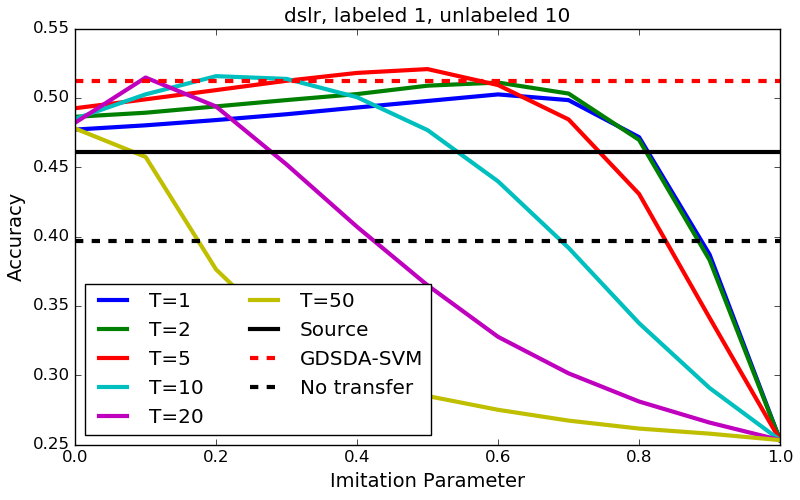
\includegraphics[width=0.3\textwidth]{figure/dslrtoamazonlabeled1unlabeled10.png}}&
\subfloat[D $\rightarrow$ A, 15 unlabeled ]{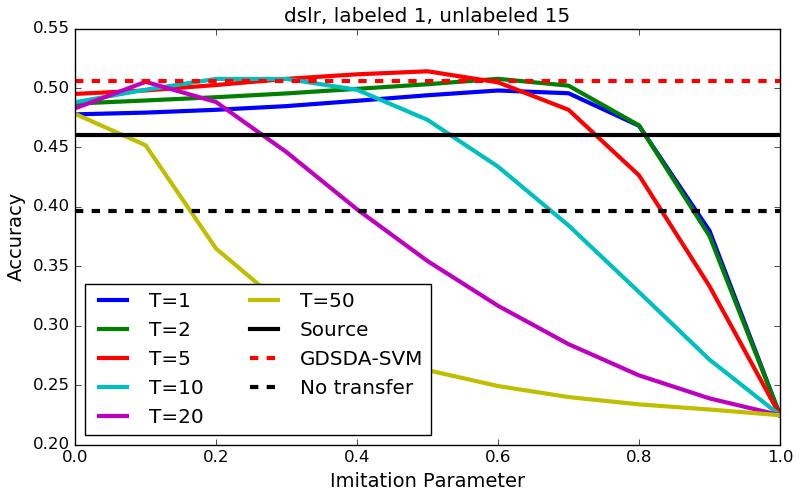
\includegraphics[width=0.3\textwidth]{figure/dslrtoamazonlabeled1unlabeled15.png}}&
\subfloat[D $\rightarrow$ A, 20 unlabeled ]{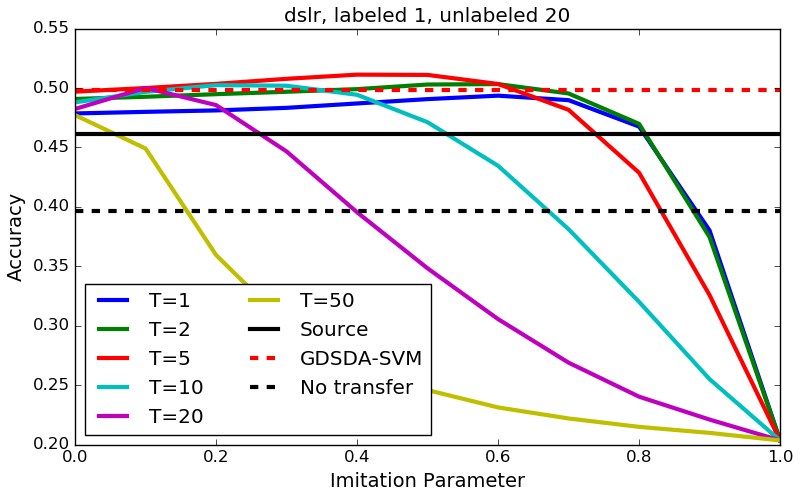
\includegraphics[width=0.3\textwidth]{figure/dslrtoamazonlabeled1unlabeled20.png}}\\
\subfloat[W $\rightarrow$ A, 10 unlabeled ]{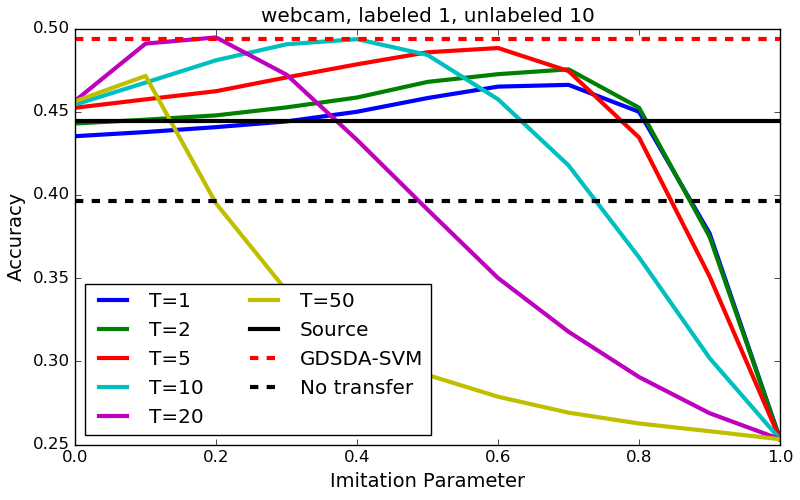
\includegraphics[width=0.3\textwidth]{figure/webcamtoamazonlabeled1unlabeled10.png}}&
\subfloat[W $\rightarrow$ A, 15 unlabeled ]{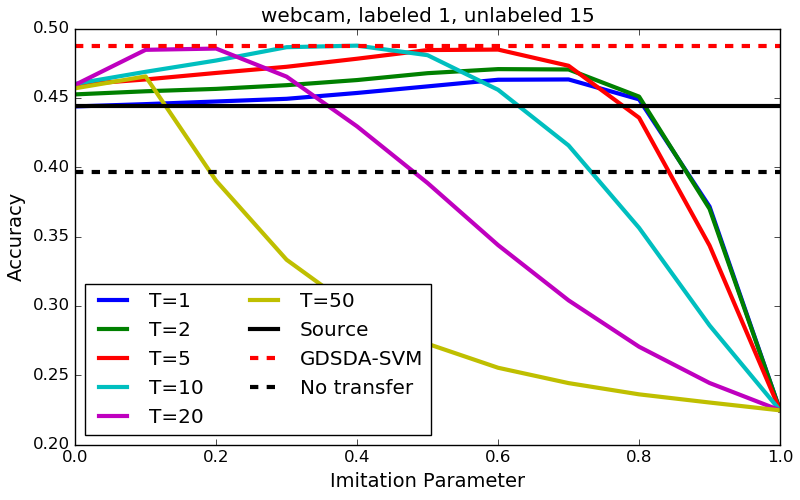
\includegraphics[width=0.3\textwidth]{figure/webcamtoamazonlabeled1unlabeled15.png}}&
\subfloat[W $\rightarrow$ A, 20 unlabeled ]{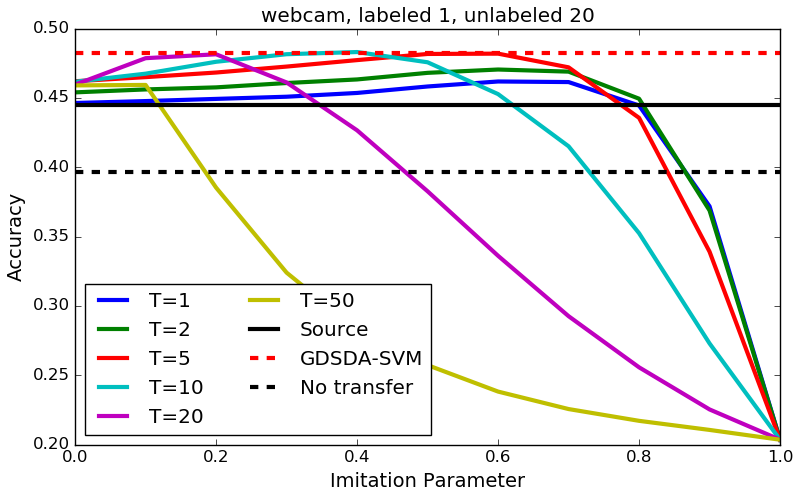
\includegraphics[width=0.3\textwidth]{figure/webcamtoamazonlabeled1unlabeled20.png}}\\
\end{tabular}
\caption{Experiment results on DSLR$\rightarrow$Amazon and Webcam$\rightarrow$Amazon when there are just one labeled examples per class. The results of DSLR$\rightarrow$Amazon and Webcam$\rightarrow$Amazon are shown in figure (a)-(c) and (d)-(e) respectively. GDSDA-SVM is trained with temperature $T=20$. The X-axis denotes the imitation parameter of the hard label (i.e. $\lambda_1$ in Fig \ref{fig:GDSDA}) and the corresponding imitation parameter of the soft label is set to $1-\lambda_1$.
}\label{fig:single1}
\end{figure}
\subsection{Multi-Source for Office datasets}
\begin{figure}
	\centering
	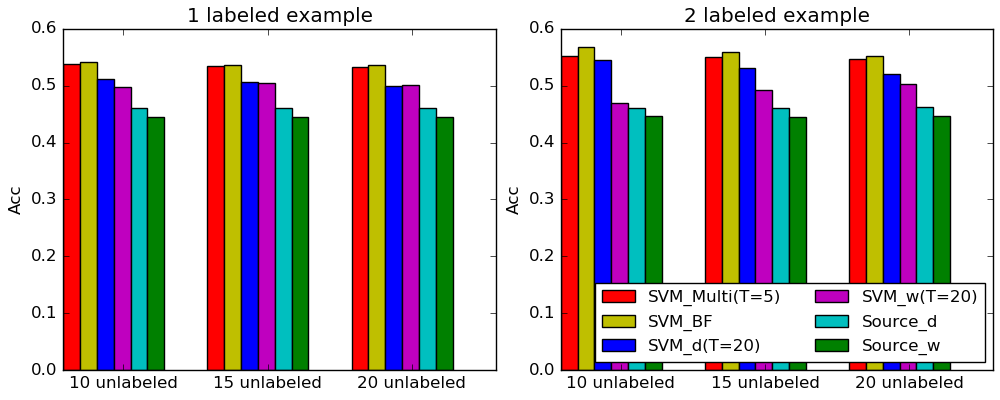
\includegraphics[scale=.34]{figure/cmp.png}
	\caption{D+W$\rightarrow$A, Multi-source results comparison.}\label{fig:multi}
\end{figure}
In this experiment, we show the performance of GDSDA-SVM under the multi-source SDA scenario.
Specifically, we use Amazon as the target domain and the target domain can leverage the knowledge of two source models trained from Webcam and DSLR.
We use the similar settings as our single source experiment and perform 2 groups of experiments using 1 labeled and 2 labeled examples per class respectively. We use temperature $T=5$ and set and $\beta=1$. The results of multi-source GDSDA-SVM are denoted as SVM\_Multi. Here we also include two single source GDSDA-SVMs obtained from the experiments above (SVM\_w and SVM\_d trained using Webcam and DSLR as the source respectively) as the baselines. Moreover, we show the best performance of the brutal force search model (SVM\_BF). For SVM\_BF, we search temperature in range $T=[1,2,5,10,20,50]$ and each imitation parameter in range $[0,0.1,...,1]$. The experiment results are shown in Figure \ref{fig:multi}.

From the results, we can see that, given 2 source models, SVM\_Multi can outperform any single source model trained with GDSDA. This indicates GDSDA-SVM can still exploit the knowledge even in the complex multi-source scenario. Even though SVM\_Multi performs slightly worse than the best result found by brutal force search in some experiments, considering their time consumption (GDSDA-SVM is around 30 times faster than brutal force search), SVM\_Multi still has its advantage in real applications.




